Como conclusión general, podemos ver como los cambios en ASM y C se pronuncian en cada uno de los filtros. Así vemos como poder trabajar a más bajo nivel para situaciones específicas puede resultar muy beneficioso si lo que buscamos es optimizar los tiempos, como contraparte es más complejo trabajar en ASM que en C.


\subsection{Tres Colores y Cambia Color}

En estos dos filtros encontramos similitudes con respecto a los tiempos de corrida. 
Se puede observar en el siguiente gráfico como sus tiempos se asemejan bastante entre sí, a pesar de ser diferentes filtros. 

\vspace{6px}
\begin{center}
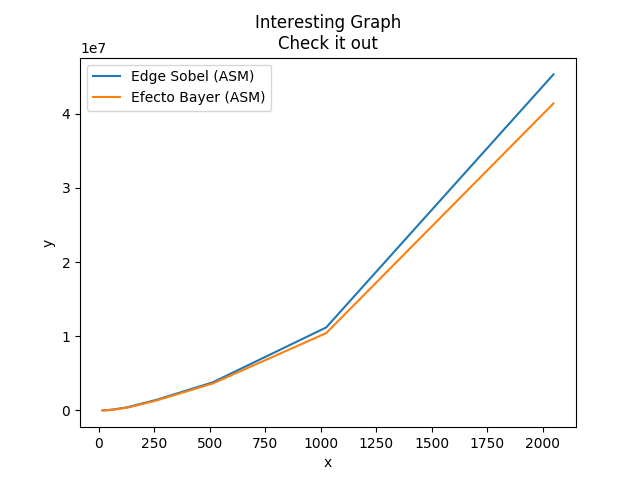
\includegraphics[width=12.5cm, height=9
cm]{images/cambia_tres.png}
\end{center}
\vspace{6px}


Uno de los primeros enfoques que surgieron a partir de esta comparación es revisar el código de cada uno de los filtros y pensar que tan complejas son las intrucciones que realiza. 
Ambos filtros tienen instrucciones como $shuffle$ que tienen un costo mucho mayor a instrucciones mas sencillas como $pand$ o $padd$. Cabe destacar también, que ambos filtros realizan pocos accesos a memoria. Esto es clave a la hora de hablar de tiempos de ejecución, ya que el tiempo que se tarda en ir a la memoria es mucho mayor a solamente trabajar dentro de registros del procesador por la proximidad de los mismos. 



\subsection{Edge Sobel y Efecto Bayer}

Sobre estos filtros también encontramos similitudes en tiempos de ejecución. Ambos filtros realizan instrucciones en general sencillas, con pocos $shuffle$ y sin conversiones de datos. Podemos ver en el siguiente gráfico las similitudes:


\vspace{6px}
\begin{center}
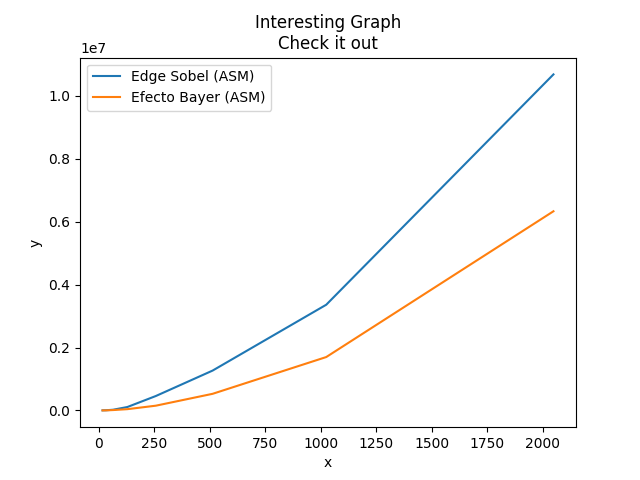
\includegraphics[width=12.5cm, height=9
cm]{images/sobel_bayer.png}
\end{center}
\vspace{6px}


A partir de estos resultados y sabiendo que las instrucciones que se realizan en ambos filtros son de "costos similares", a pesar de no tener la misma cantidad de instrucciones, podemos ver como los tiempos se asemejan lo suficiente como para pensar que es por la similitud en complejidad de dichas instrucciones. Esto significa que ambas tienen tiempos similares debido a que ambas utilizan instrucciones poco costosas de ASM. 


\subsection{Sobre los 4 filtros}

Como una conclusón general nos gustaría hacer una comparación entre $Cambia$ $Color$ y $Tres$ $Colores$ contra $Edge$ $Sobel$ y $Efecto$ $Bayer$. 
Entre ambos grupos podemos notar una diferencia grande en los tiempos de ejecución en ASM. 
Nuestro principal hipótesis sobre dicha diferencia en las complejidad de las intrucciones que tienen a cargo cada uno de los grupos de filtros. En el primero grupo ($Cambia$ $Color$ y $Tres$ $Colores$) tenemos instrucciones como $shuffle$ que a diferencia del segundo grupo ($Edge$ $Sobel$ y $Efecto$ $Bayer$) no se encuentran tan seguido en cada iteración como en el primer grupo. Otro punto a destacar sobre el mismo eje son las conversiones de datos, en el segundo grupo no se realiza ninguna conversión de datos a diferencia del primero, donde de momento se trabaja en $int$ y en otros necesitamos la precisión de los $floats$. 